\chapter{Analýza}
\label{analysis-and-its-results}

V tejto sekcií popisujem výsledky mojej analýzy nasadenia technológie NEL. 
Najskôr uvádzam, aké dáta sa mi podarilo získať a ako som s nimi pracoval.
Potom prezentujem všetky získané znalosti.

\section{Získané HTTP Archive dáta}
\label{result-data}

S implementovanými nástrojmi som začal vykonávať analýzu postupne. Najskôr podľa postupu z predošlej analýzy, aby som overil správnosť nových nástrojov pre vykonávanie tej mojej.
Stiahol som teda HTTP Archive dáta pre všetky februárové mesiace za skúmané obdobie.

Po otestovaní nástrojov a konzultácií priebežných výsledkov s vedúcim práce som začal analyzovať všetky mesiace od februára 2018 až po február 2023.
V rámci tohto skúmaného rozsahu som zistil, že HTTP Archive z nejakého dôvodu neobsahuje za mesiace máj a jún v roku 2022 žiadne NEL hlavičky 
v žiadnom z uložených zdrojov. 
To znamená, že za tie mesiace nie sú v zdrojových dátach žiadne údaje o stave nasadenia NEL.
Taktiež som zistil, že pre január 2019 neexistujú žiadne HTTP Archive dáta.
To, že tieto dáta chýbajú sa zobrazilo na výsledných metrikách.

Analýzu som v neskoršom štádiu práce dokončil aj na zvyšných dátach, teda od marca 2023 do apríla 2024.
Uchoval som všetky dáta, ktoré som z HTTP Archive stiahol pomocou na to určeného nástroja (viď sekciu \ref{query_and_store}). 

\section{Vypočítané metriky}

Z uvedených dát som získal výsledky celkovej práce použitím nástroja pre výpočet preddefinovaných metrík (viď sekciu \ref{analyze_results}).
Poradilo sa mi vypočítať všetky zo spomínaných metrík (viď vstupy a výstupy práce v kapitole \ref{possible-analysis-strategies}).

\subsection{Domény používajúce NEL}

Pri pohľade na celé skúmané obdobie, počet domén používajúcich NEL od publikácie jeho špecifikácie do apríla 2024 vzrástol na približne 2.6 milióna. 
Túto skutočnosť popisuje obrázok \ref{fig:httparchive-nel-deployment}, kde je vykreslený približný počet domén používajúcich NEL pre každý skúmaný mesiac.
Podľa tohto obrázka je možné vyčítať, že značné nárasty vo využívaní analyzovanej technológie sa udiali v mesiacoch november 2018, apríl 2019, október 2020 a august 2022.
Naopak najbadateľnejšie poklesy vo využívaní sa udiali v mesiacoch január 2021, október 2021 a v decembri 2023.

\begin{figure}[!htb]
\begin{center}
 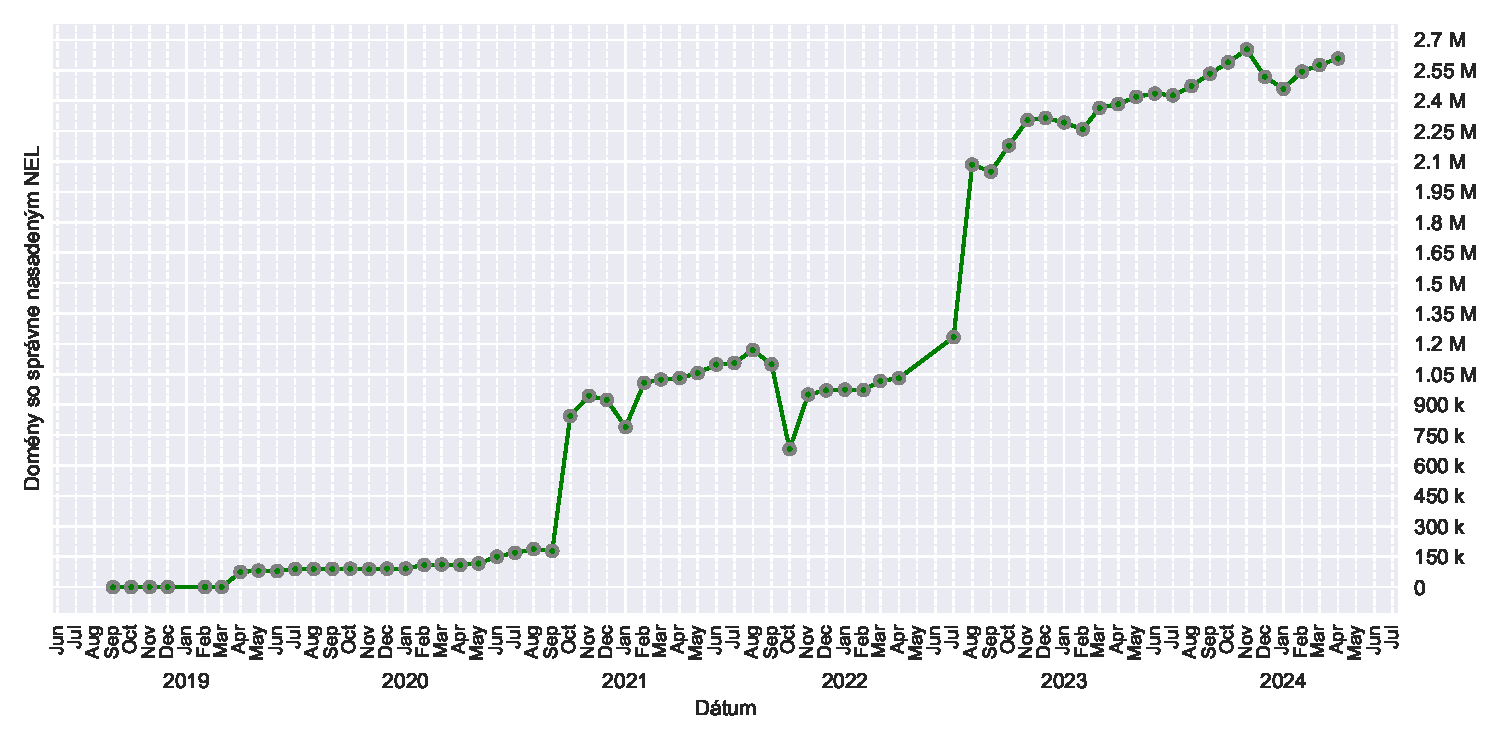
\includegraphics[scale=0.59]{obrazky-figures/httparchive_nel_deployment.pdf}
 \caption{Graf zobrazujúci rast počtu domén so správne nasadenou technológiou NEL.}
 \label{fig:httparchive-nel-deployment}
\end{center}
\end{figure}

Pre pohľad na presné počty po jednotlivých mesiacoch som ďalej zhotovil graf uvedený v obrázku \ref{fig:httparchive-nel-deployment_ratio_values}.
Je v ňom pre každý mesiac počas všetkých rokov uvedený počet domén so správne nasadeným NEL (prvé číslo pre daný mesiac) a celkový počet skúmaných domén (druhé číslo pre daný mesiac). 
Z neho je možné vyčítať doplnkové informácie:
\begin{itemize}
    \item počiatočný počet skúmaných domén bol 2 096 799, 
    \item počet skúmaných domén v poslednom skúmanom mesiaci bol 20 424 419,
    \item počiatočné percentuálne nasadenie NEL bolo 0.000095\%,
    \item percentuálne nasadenie NEL v poslednom skúmanom mesiaci bolo 12.77\%,
    \item presný počet domén pri výrazných nárastoch a poklesoch v nasadení NEL:
    \begin{itemize}
        \item november 2018 -- nárast z 10 domén na 187,
        \item apríl 2019 -- nárast z 382 domén na 74 590,
        \item október 2020 -- nárast z 178 670 domén na 844 665,
        \item január 2021 -- pokles z 923 400 domén na 789 667,
        \item október 2021 -- pokles z 1 099 507 domén na 680 909,
        \item august 2022 -- nárast z 1 233 049 domén na 2 084 724,
        \item december 2023 -- pokles z 2 653 529 domén na 2 518 117.
    \end{itemize}
\end{itemize}

Na tomto grafe, tak ako aj na niekoľkých ďalších, sa prejavil výpadok dát za mesiace máj a jún v roku 2022.
Pre tie mesiace platí, že žiadne NEL domény v dátach HTTP Archive jednoducho nájdené neboli. 
To platí zároveň pre všetky ostatné mesiace, ku ktorým prislúcha iba číslo 0.

Podarilo sa mi tiež zistiť príčiny niektorých z vyššie zmienených nárastov v počte domén s nasadeným NEL.
Vysvetlené sú v nasledujúcej sekcii.

\begin{figure}[!htb]
\begin{center}
 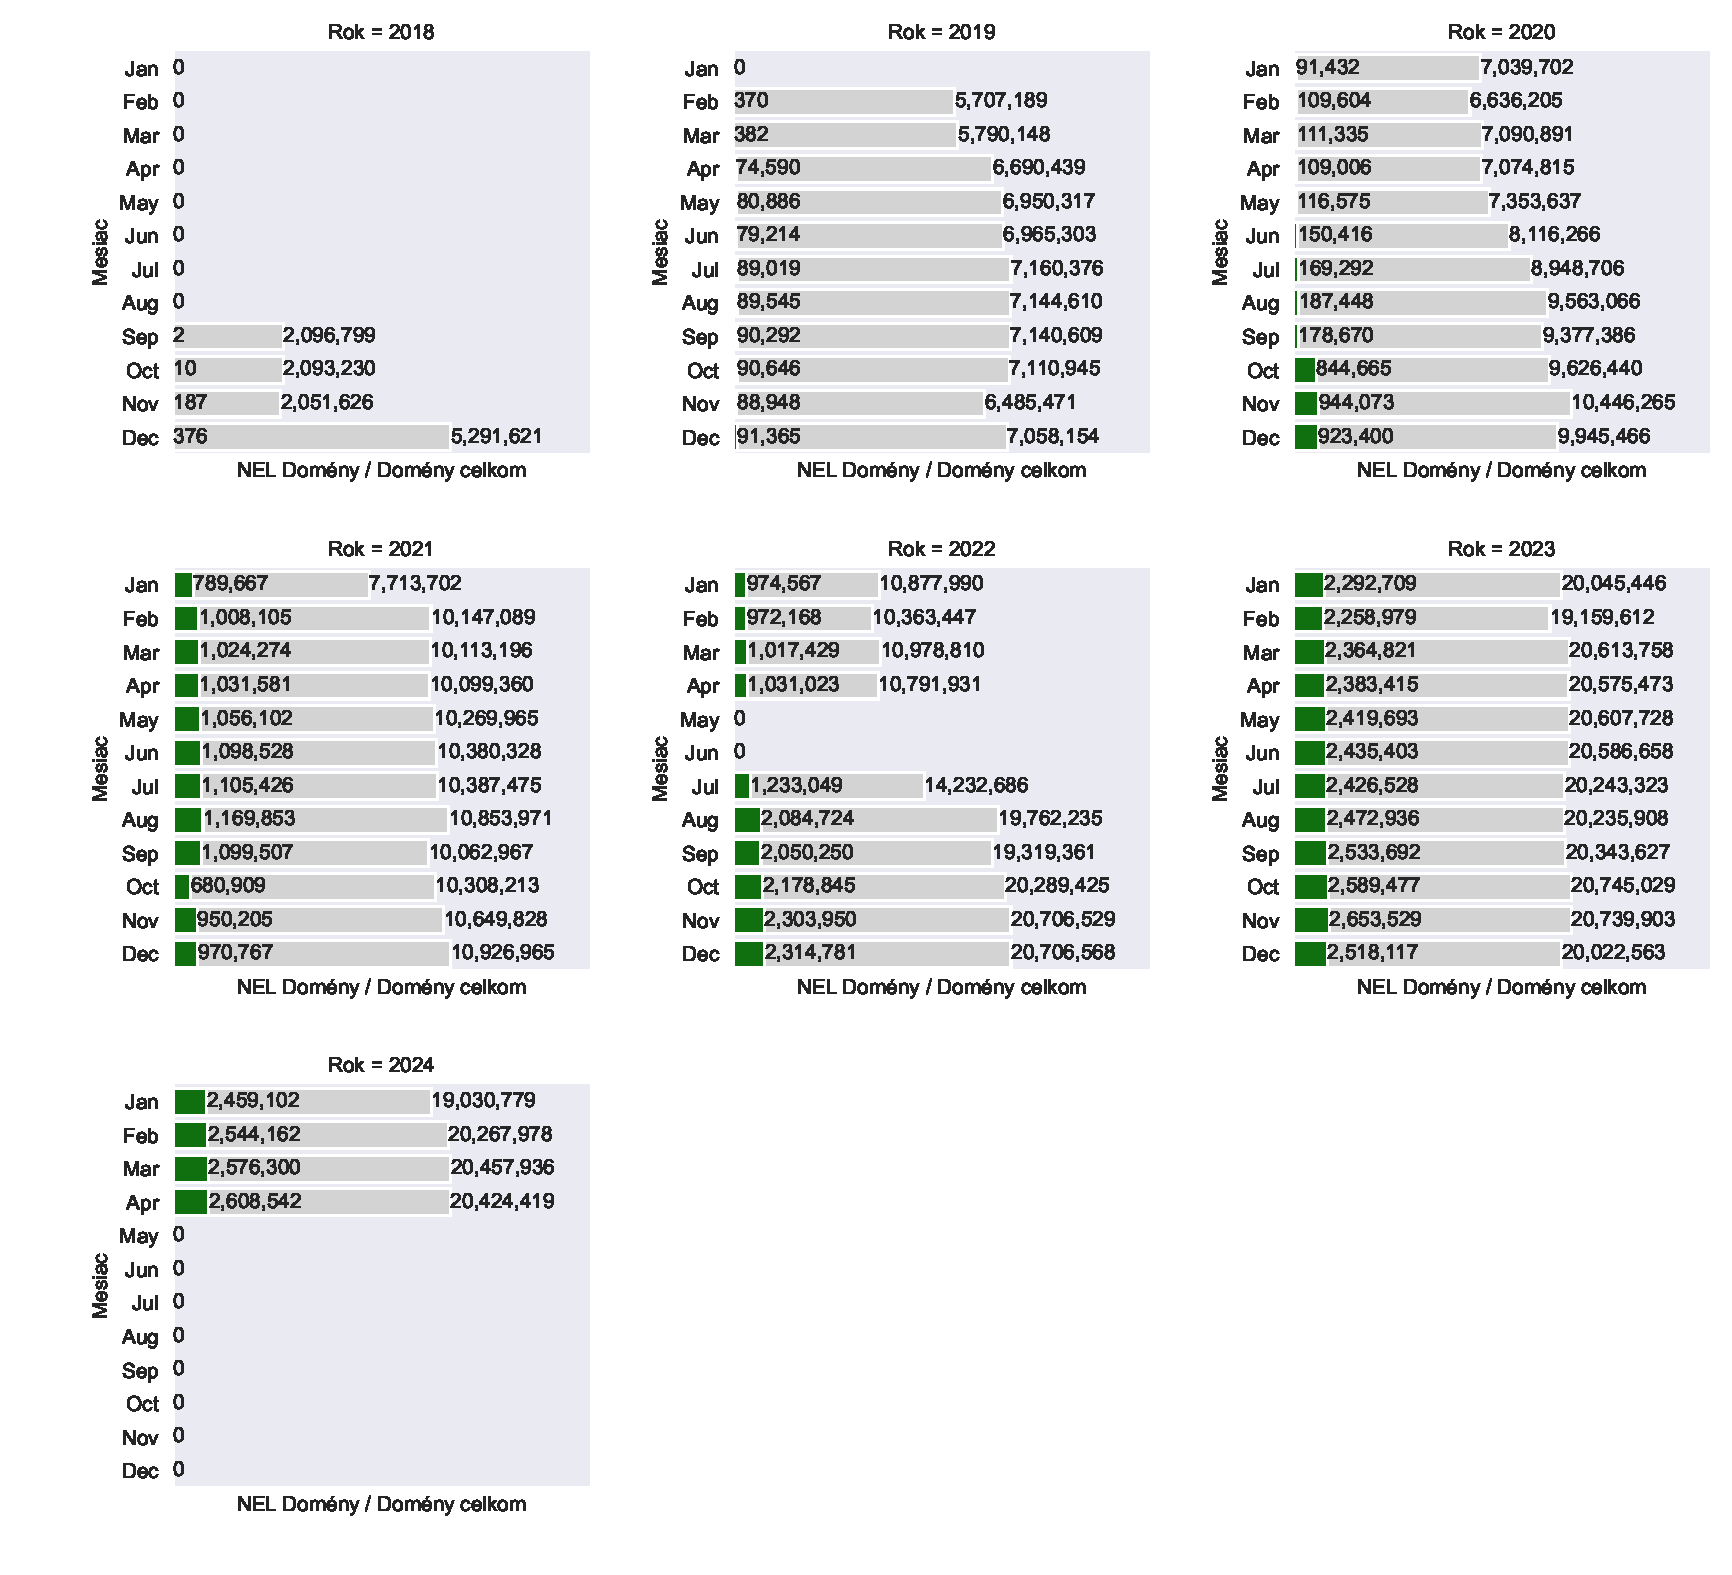
\includegraphics[scale=0.518]{obrazky-figures/httparchive_nel_deployment_ratio_values.pdf}
 \caption{Graf zobrazujúci presné počty domén so správne nasadenou technológiou NEL \mbox{v porovnaní} s celkovým počtom preskúmaných domén za jednotlivé mesiace.}
 \label{fig:httparchive-nel-deployment_ratio_values}
\end{center}
\end{figure}

\pagebreak


\subsection{Poskytovatelia používaných NEL kolektorov}

% TODO definovať v teórií poskytovateľa kolektorov
Počet poskytovateľov NEL kolektorov používaných počas skúmaného obdobia je pomerne malý.
Identifikoval som 425 poskytovateľov, ktoré sa za toto obdobie vyskytli.
Počet aktívnych poskytovateľov po jednotlivých mesiacoch uvádza graf v obrázku \ref{fig:httparchive-nel-collector-provider-count}.
Graf vykresľuje stabilný, postupný nárast v ich počte.
Počas tohto rastu dvakrát došlo k výraznému poklesu.
Prvý v júli 2022, hneď po výpadku HTTP Archive dát.
Druhý neskôr v marci 2023.

Z výsledných dát vypočítanej metriky pre kolektory viem, že prvým poskytovateľom NEL kolektorov bola doména \code{bingparachute.com}.
Počiatočne ho používali práve 2 jedinečné domény.
Za posledný preskúmaný mesiac bolo aktívnych presne 326 poskytovateľov.

\begin{figure}[!htb]
\begin{center}
 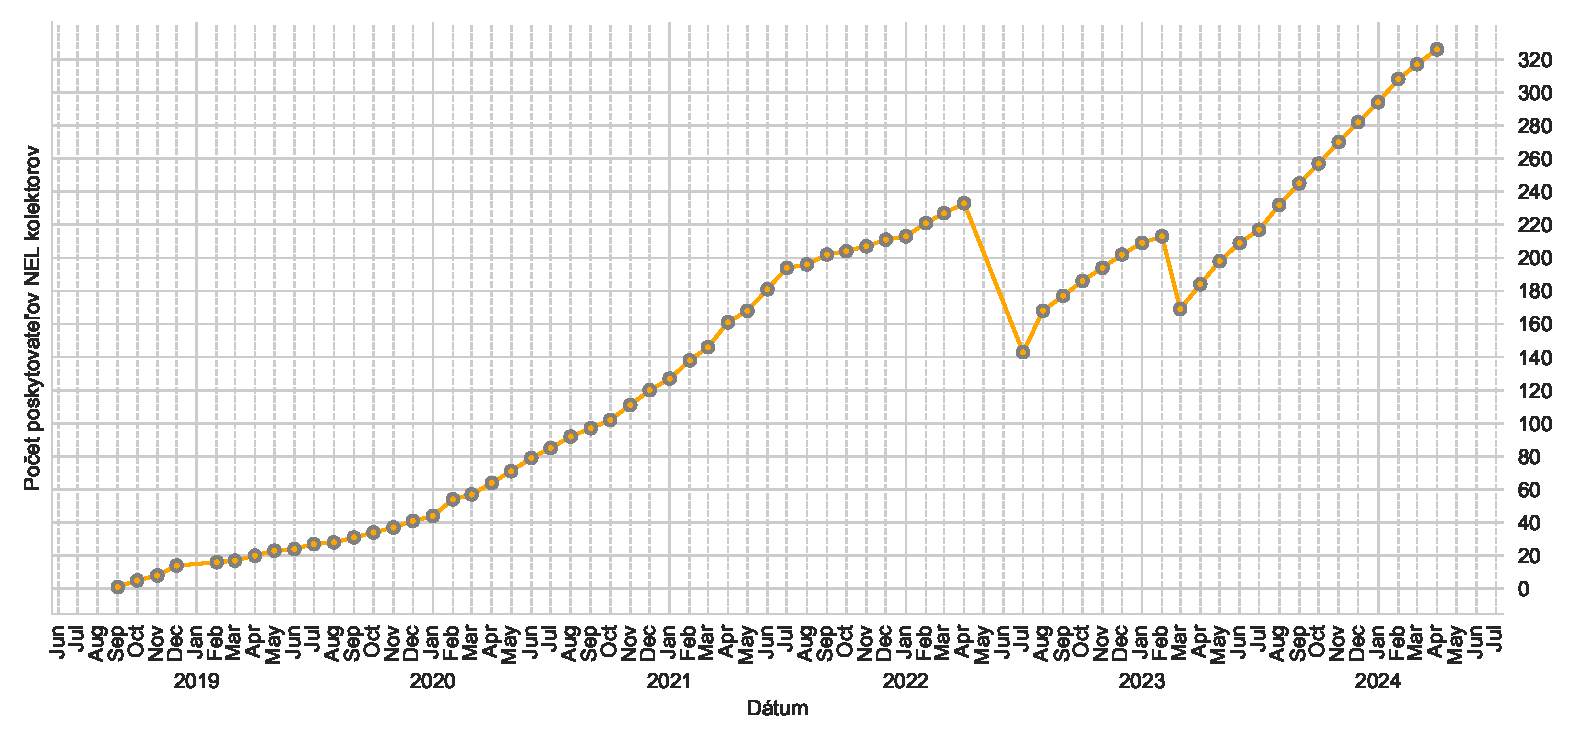
\includegraphics[scale=0.57]{obrazky-figures/httparchive_nel_collector_provider_count.pdf}
 \caption{Graf zobrazujúci rast počtu poskytovateľov NEL kolektorov.}
 \label{fig:httparchive-nel-collector-provider-count}
\end{center}
\end{figure}

Vizualizácia v obrázku \ref{fig:httparchive-nel-collector-provider-top-1-over-time} zobrazuje poskytovateľov NEL kolektorov s najvyšším počtom obsluhovaných domén za skúmané obdobie. 
Vďaka tomuto grafu som zistil, že tie najviac badateľné nárasty v počte domén využívajúcich NEL sú spojené s príchodom konkrétnych poskytovateľov NEL kolektorov:
\begin{itemize}
\item november 2018 -- nárast spôsobený kolektormi od \code{report-uri.com},
\item apríl 2019 -- nárast spôsobený kolektormi od \code{shopifycloud.com},
\item október 2020 -- nárast spôsobený kolektormi od \code{cloudflare.com},
\item august 2022 -- nemožno určiť podľa obrázka \ref{fig:httparchive-nel-collector-provider-top-1-over-time}.
\end{itemize}

\begin{figure}[!htb]
\begin{center}
 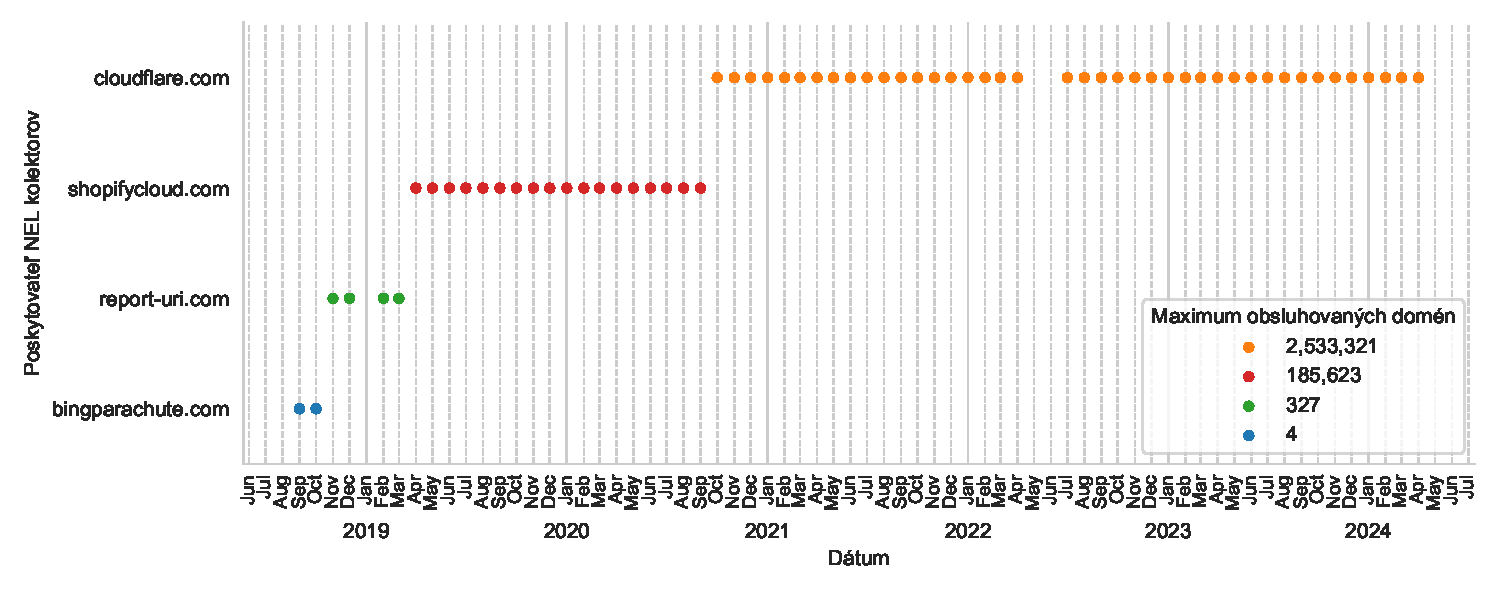
\includegraphics[scale=0.598]{obrazky-figures/httparchive_nel_collector_provider_top_1_over_time.pdf}
 \caption{Identifikácia dominantných poskytovateľov NEL kolektorov (s najvyšším počtom obsluhovaných domén) pre každý skúmaný mesiac. V legende grafu je priložený údaj \mbox{o maximálnom} počte obsluhovaných domén za celkové obdobie výskytu jednotlivých dominantných poskytovateľov.}
 \label{fig:httparchive-nel-collector-provider-top-1-over-time}
\end{center}
\end{figure}

\pagebreak

Nárast za august 2022 však môžem popísať dátami z použitej metriky pre graf v obrázku vyššie.
O tento nárast sa prevažne zaslúžil \code{cloudflare.com}, najpoužívanejší poskytovateľ NEL kolektorov v tom čase. 
Počet ním obsluhovaných domén totiž z júna 2022 na august 2022 narástol o 836 324.

\subsection{História hlavných poskytovateľov NEL kolektorov}

Okrem iného je zo získaných dát možné preskúmať poskytovateľov NEL kolektorov do hĺbky.
Pre rozsahové limity tejto práce som si na ukážku musel nejakým spôsobom vybrať množinu poskytovateľov na hlbší prieskum.
Cieľom bolo vybrať tých čo najviac relevantných.
\mbox{Z dát} som zistil, že sa pre každý mesiac v skúmanom období vyskytoval práve jeden značne dominantný poskytovateľ v počte obsluhovaných domén.
V prevažnej väčšine mesiacov je pomer obsluhy domén dominantným poskytovateľom k celkovej obsluhe všetkými dostupnými poskytovateľmi viac ako 90\%.
Týchto dominantných poskytovateľov už popisuje graf v obrázku \ref{fig:httparchive-nel-collector-provider-top-1-over-time} vyššie.

Ako zaujímavých som si nakoniec vybral najpoužívanejších 10 poskytovateľov za posledný mesiac v skúmanom období.
Zahŕňajú jednak toho najdominantnejšieho poskytovateľa za celé skúmané obdobie, ale aj niektorých, čo poskytujú svoje kolektory už od roku 2020 a skôr.
Znázorňuje ich tabuľka \ref{tab:top-10-latest-nel-collector-providers-stats}.

Zistil som, že iba \code{cloudflare.com} začal testovať NEL na iba jedinej obsluhovanej doméne. Naopak, maximum domén obsluhovaných v mesiaci nasadenia dosahuje \code{fandom.com}.
Poskytovateľ, ktorý sa v rámci tejto množiny objavil ako prvý je \code{report-uri.com}.
Poskytuje totiž NEL kolektory už od druhého skúmaného mesiaca za celé obdobie, konkrétne od októbra 2018.
Posledný stĺpec v tabuľke \ref{tab:top-10-latest-nel-collector-providers-stats} potvrdzuje skutočnosť, že \code{cloudflare.com} je naozaj značne dominantným poskytovateľom NEL kolektorov.
Stĺpec totiž obsahuje hodnoty reprezentujúce podiely na obsluhe celkového počtu domén s nasadeným NEL, pričom \code{cloudflare.com} má podiel skoro 96,3\%.

\begin{table}[!htb]
\centering
\resizebox{\textwidth}{!}{\begin{tabular}{ll||r|r|r|rr}
\toprule
Dátum & Poskytovateľ & D. nasadenia & Obsluha (nasadenie) & Obsluha (aktuálne) & \% z celku za mesiac \\
\midrule
\midrule
\multirow{10}{*}{Apr 2024} & cloudflare.com & Aug 2020 & 1 & 2,511,907 & 96.273 \\
& heroku.com & Aug 2023 & 2 & 45,405 & 1.740 \\
& fandom.com & May 2023 & 11 & 29,833 & 1.143 \\
& freshedge.net & Oct 2022 & 5,772 & 8,999 & 0.345 \\
& dz8aopenkvv6s.cloudfront.net & Aug 2022 & 2,552 & 3,829 & 0.147 \\
& wikimedia.org & Sep 2020 & 27 & 1,447 & 0.055 \\
& hhdev.ru & Aug 2021 & 120 & 1,385 & 0.053 \\
& report-uri.com & Oct 2018 & 3 & 1,190 & 0.046 \\
& yandex.net & May 2020 & 19 & 1,082 & 0.041 \\
& gumlytics.com & Dec 2021 & 7 & 610 & 0.023 \\
\bottomrule
\end{tabular}}
\caption{Detaily pre 10 najpoužívanejších poskytovateľov NEL kolektorov za apríl 2024.}
\label{tab:top-10-latest-nel-collector-providers-stats}
\end{table}

Ďalej v obrázku \ref{fig:httparchive-nel-latest-collector-provider-stats} uvádzam graf vizualizujúci približné počty mesačne obsluhovaných domén týmito poskytovateľmi. 
Z grafu je možné vyčítať ako sa od prvého mesiaca funkčnosti daného poskytovateľa menil počet domén, ktoré obsluhuje.
V mesiacoch máj a jún 2022 sa nejedná o prerušenie dostupnosti jednotlivých poskytovateľov, ale o zmienenú absenciu NEL hlavičiek v HTTP Archive dátach.

\begin{figure}[!htb]
\begin{center}
 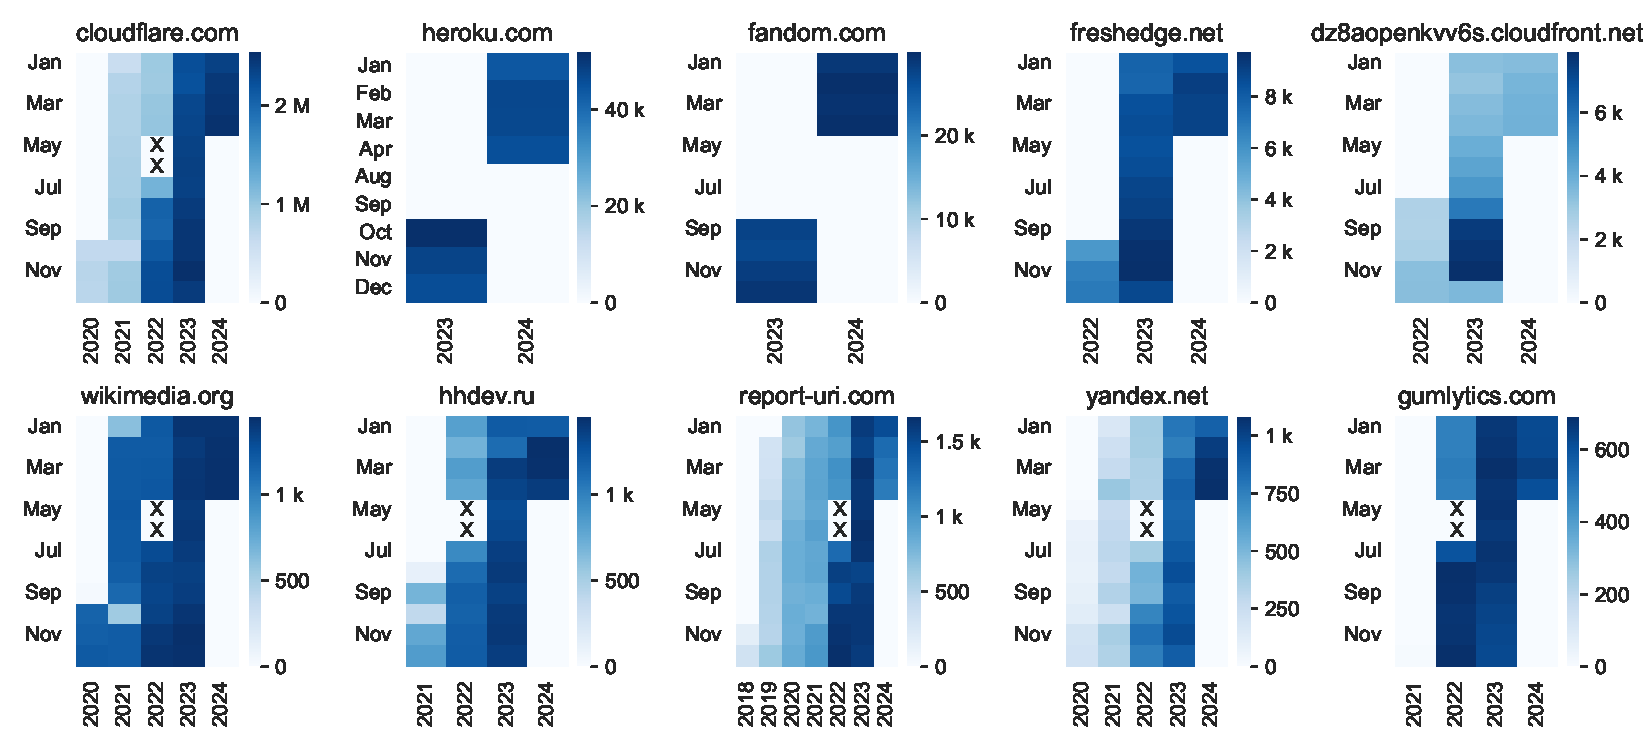
\includegraphics[scale=0.54]{obrazky-figures/httparchive_nel_latest_collector_provider_stats.pdf}
 \caption{Vývin v počte obsluhovaných domén pre 10 najpoužívanejších poskytovateľov NEL kolektorov detegovaných v apríli 2024. Znakom \code{X} sú v grafe vyznačené mesiace, pre ktoré chýbali v dátach záznamy NEL.}
 \label{fig:httparchive-nel-latest-collector-provider-stats}
\end{center}
\end{figure}

\pagebreak

\subsection{Konfigurácie}

Konfigurácia NEL pozostáva z nastavenia hodnôt pre štyri polia HTTP hlavičky \code{NEL}. Ide o \code{include\_subdomains}, \code{failure\_fraction}, \code{success\_fraction} a \code{max\_age}.

Na základe toho som zhotovil grafy, ktoré sledujú rôzne hodnoty týchto polí počas skúmaného obdobia.

Prvý graf v obrázku \ref{fig:httparchive-nel-config-is-dist} reprezentuje nastavenie poľa \code{include\_subdomains}.
Hodnota \code{true} pre toto pole prevládala od počiatku využívania NEL až do marca 2019.
Odvtedy jednoznačne začala prevládať hodnota \code{false}.
Graf na ose Y vykresľuje hodnoty v logaritmickej škále.

\begin{figure}[!htb]
\begin{center}
 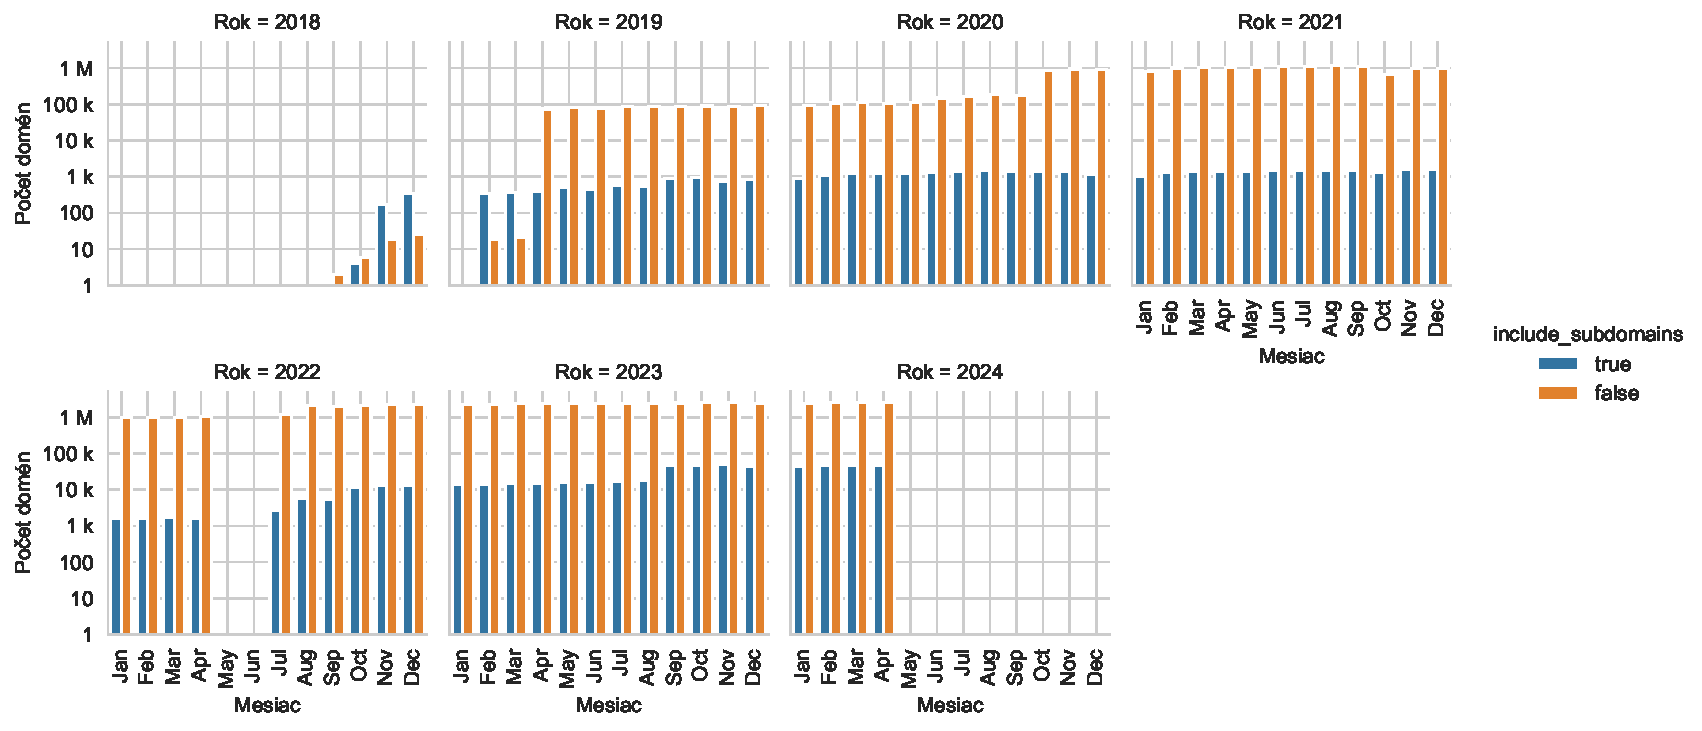
\includegraphics[scale=0.525]{obrazky-figures/httparchive_nel_config_is_dist.pdf}
 \caption{Hodnoty konfiguračného poľa \code{include\_subdomains} počas skúmaného obdobia.}
 \label{fig:httparchive-nel-config-is-dist}
\end{center}
\end{figure}

\pagebreak

Hodnotami pre zvyšné konfiguračné polia sú reprezentácie čísel.
Pre prezentovanie týchto hodnôt som ich rozdelil do intervalov.
Hraničné hodnoty jednotlivých intervalov som zvolil tak, aby reprezentovali často používané hodnoty pre dané konfiguračné pole.

Graf pre pole \code{failure\_fraction} uvádza obrázok \ref{fig:httparchive-nel-config-ff-dist}.
Jednoznačne najviac používaná hodnota tohto poľa je \code{1.0}.
To však platí až od druhej polovice roku 2020. 
Do tej doby bolo najpoužívanejšou hodnotou \code{0.01}.
Naopak, hodnoty v rozmedzí od \code{0.05} až \code{0.10} neboli používané nikdy a hodnota \code{0.00} sa za celý čas vyskytla iba raz.

\begin{figure}[!htb]
\begin{center}
 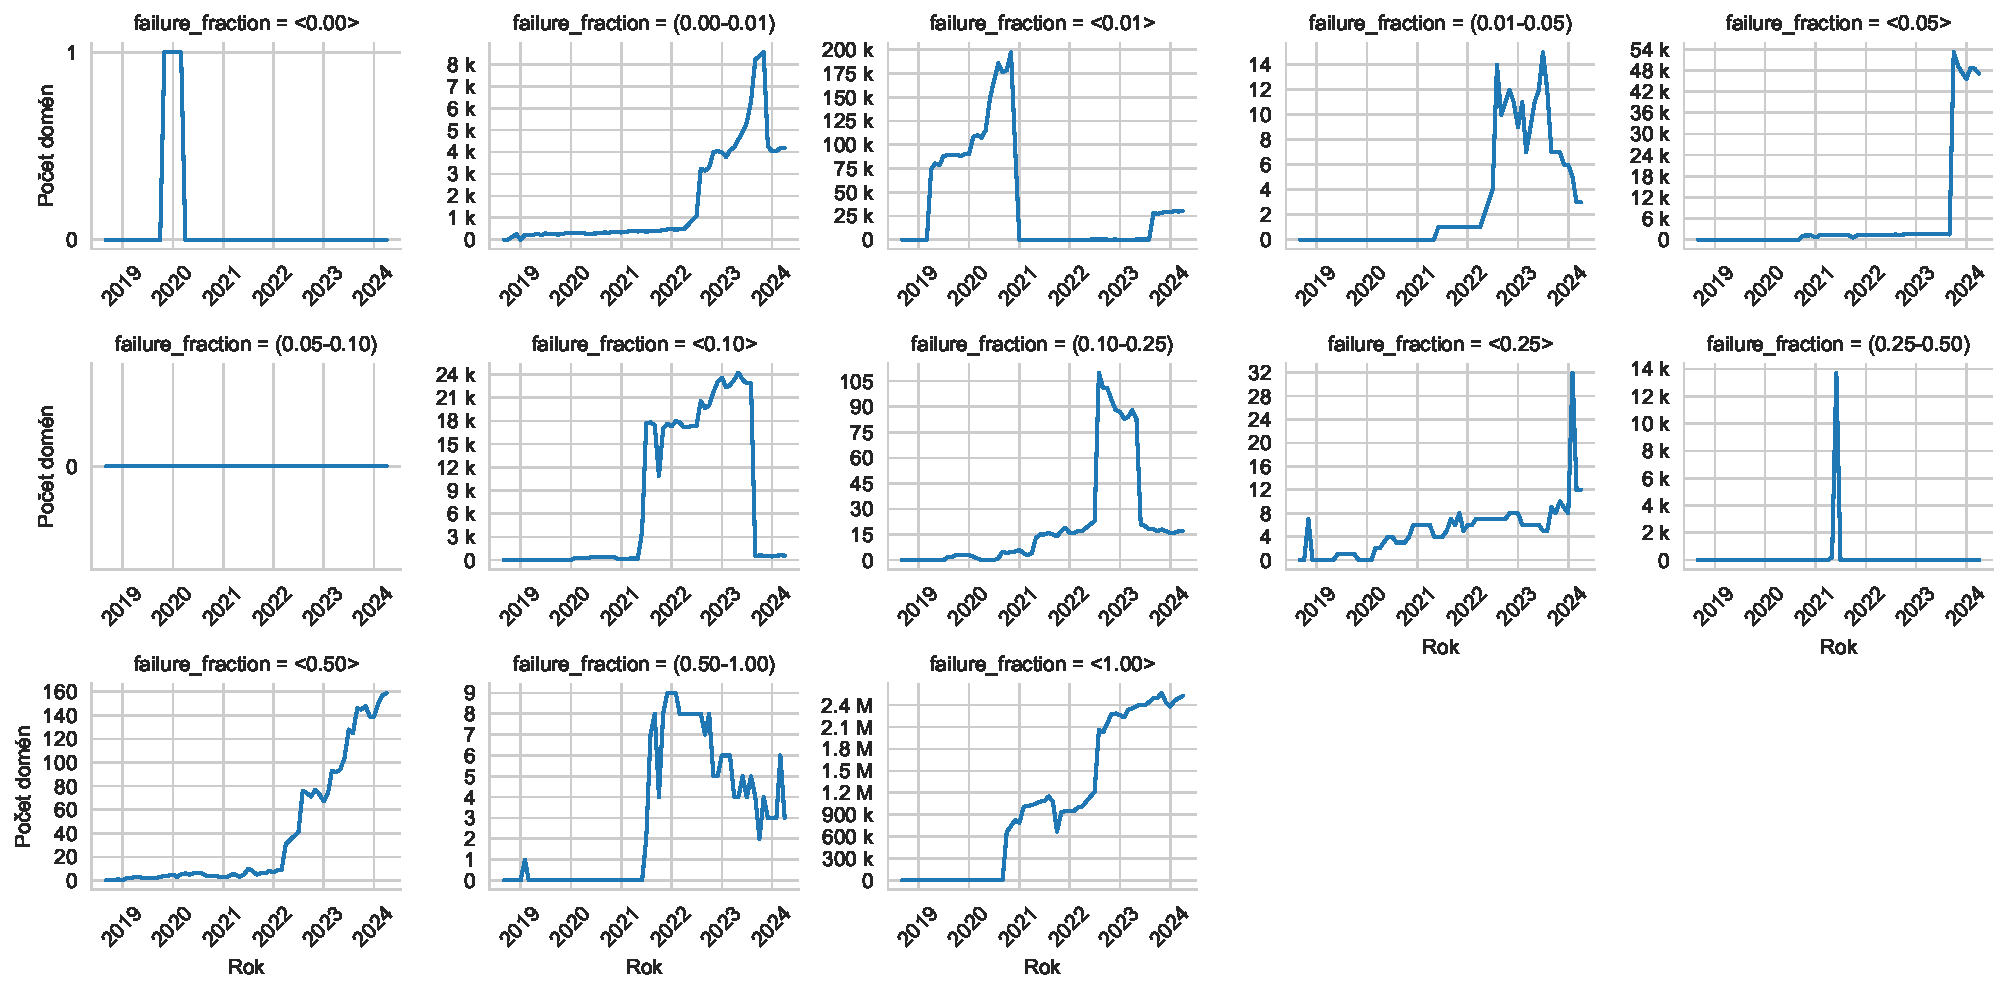
\includegraphics[scale=0.447]{obrazky-figures/httparchive_nel_config_ff_dist.pdf}
 \caption{Hodnoty konfiguračného poľa \code{failure\_fraction} počas skúmaného obdobia.}
 \label{fig:httparchive-nel-config-ff-dist}
\end{center}
\end{figure}

Graf pre ďalšie pole, \code{success\_fraction} je v obrázku \ref{fig:httparchive-nel-config-sf-dist}. 
Prevláda tu hodnota \code{0.00}.

\begin{figure}[!htb]
\begin{center}
 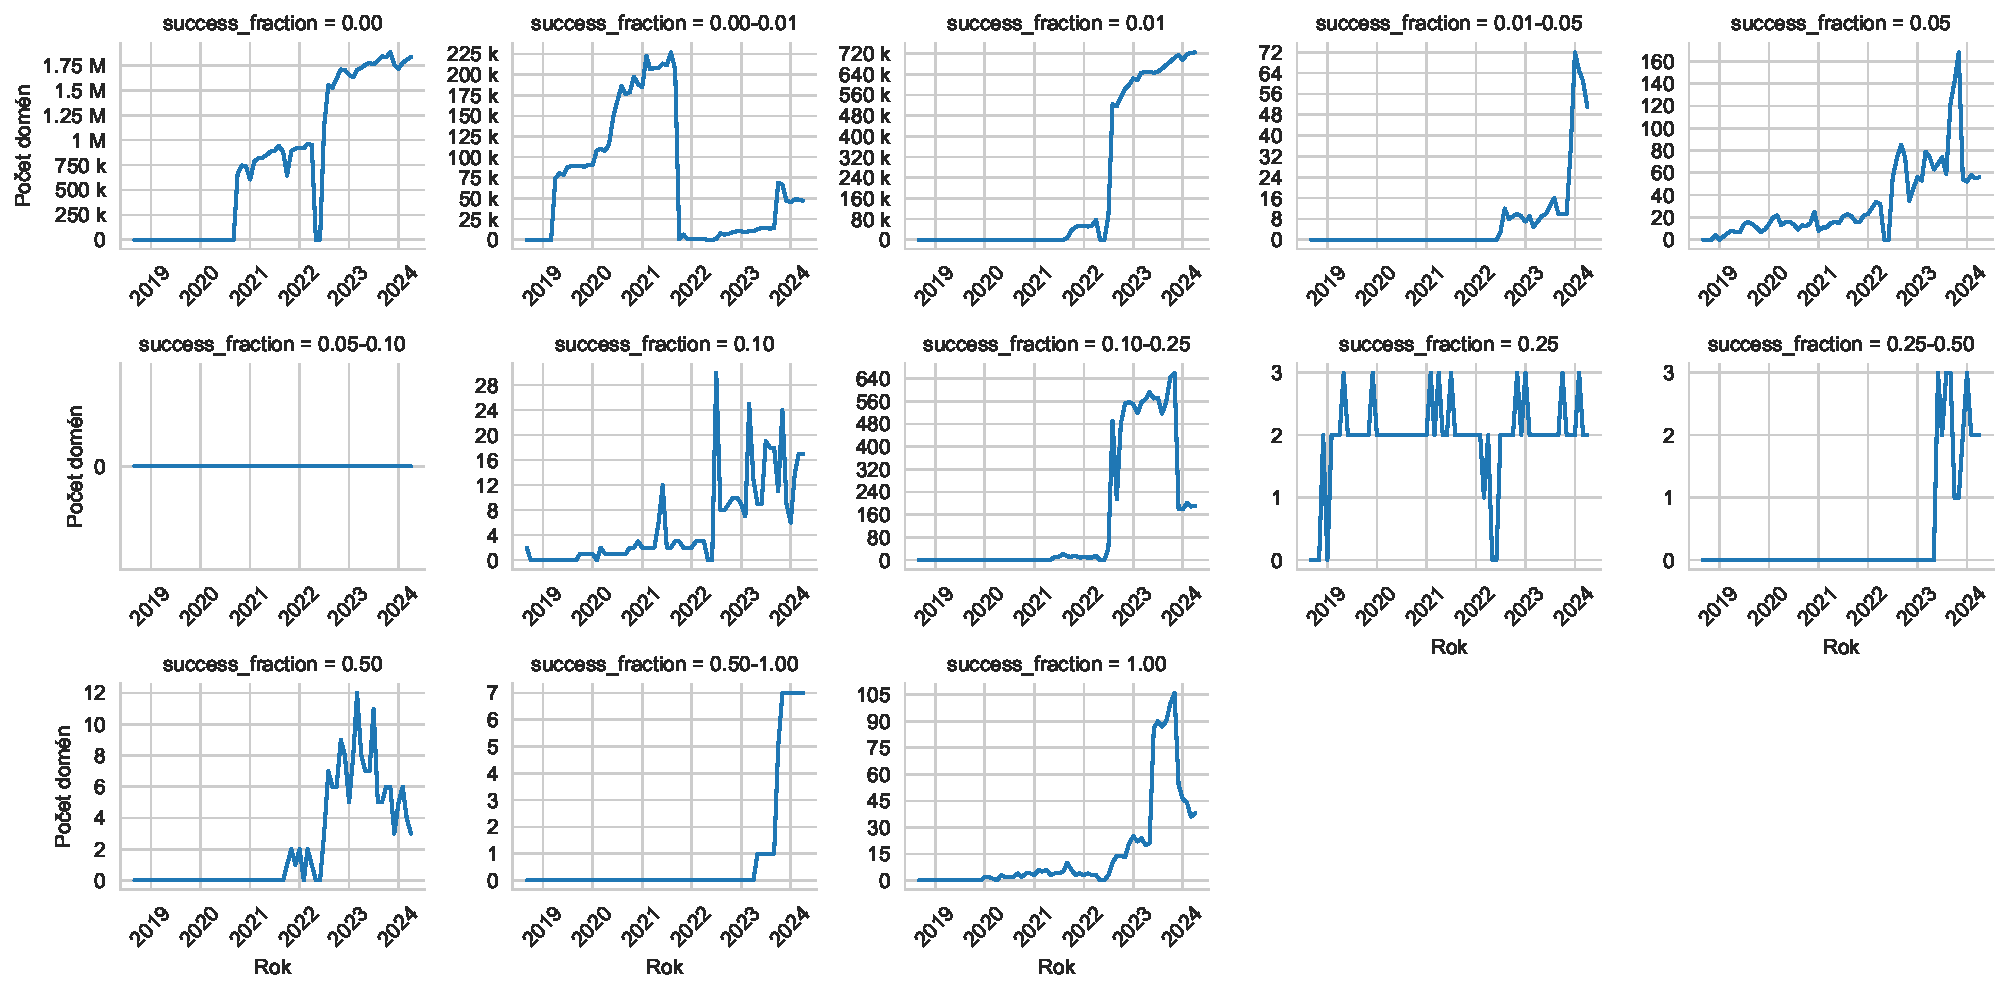
\includegraphics[scale=0.447]{obrazky-figures/httparchive_nel_config_sf_dist.pdf}
 \caption{Hodnoty konfiguračného poľa \code{success\_fraction} počas skúmaného obdobia.}
 \label{fig:httparchive-nel-config-sf-dist}
\end{center}
\end{figure}

\pagebreak

Okrem najčastejšej hodnoty je pre \code{success\_fraction} najzastúpenejšou voľbou \code{0.01}, alebo hodnoty v rozmedzí od \code{0.00} do \code{0.01}.
Zvyšné intervaly hodnôt sa nepoužívajú skoro vôbec.

Posledné pole, \code{max\_age} popisuje graf v obrázku \ref{fig:httparchive-nel-config-ma-dist}.
Prevládajú nastavenia na hodnoty \code{604800}, teda 7 dní v sekundách, alebo \code{2592000}, čo predstavuje 30 dní v sekundách.

\begin{figure}[!htb]
\begin{center}
 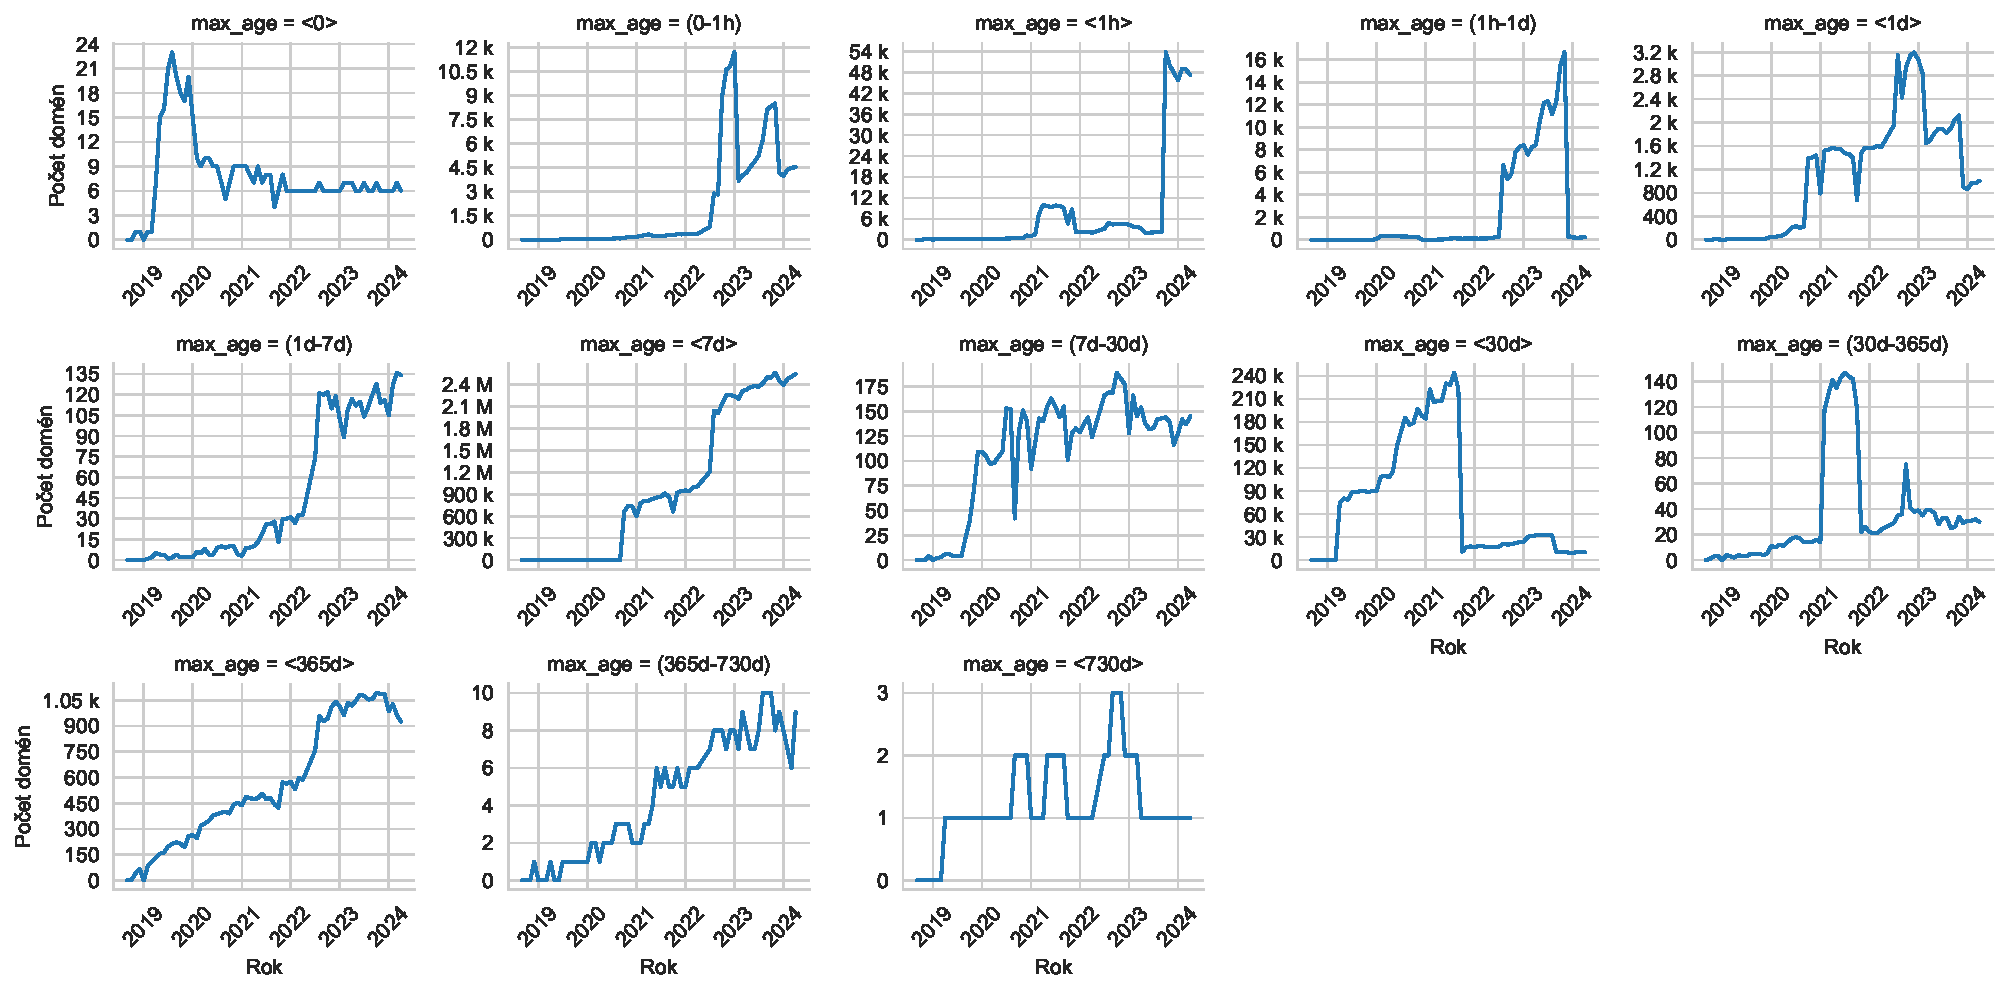
\includegraphics[scale=0.447]{obrazky-figures/httparchive_nel_config_ma_dist.pdf}
 \caption{Hodnoty konfiguračného poľa \code{max\_age} počas skúmaného obdobia.}
 \label{fig:httparchive-nel-config-ma-dist}
\end{center}
\end{figure}

Okrem používanosti samostatných hodnôt som zistil aj aké nastavenia celkovej konfigurácie prevažovali za jednotlivé mesiace.
V tabuľke \ref{tab:nel_config_popular_annual_config} uvádzam najviac vyskytujúce sa variácie konfigurácie NEL za vybrané mesiace.
Pre túto tabuľku som si vybral koniec každého roka a ako posledný riadok som pridal aj posledný mesiac skúmaného obdobia, apríl 2024.
Podľa predošlých grafov je z tejto tabuľky možné vyčítať, že sa s jednoznačnou prevahou používajú v každom zvolenom mesiaci tie najpoužívanejšie hodnoty samostatných polí z daného obdobia.

\begin{table}[!htb]
\centering
\resizebox{\textwidth}{!}{
\begin{tabular}{l||r|r|r|r|r}
\toprule
Dátum & \code{include\_subdomains} & \code{failure\_fraction} & \code{success\_fraction} & \code{max\_age} & Počet domén \\
\midrule
\midrule
Dec 2018 & true & 0.00001 & 0.0 & 3600 & 249 \\
Dec 2019 & false & 0.01 & 0.0001 & 2592000 & 90,373 \\
Dec 2020 & false & 1.0 & 0.0 & 604800 & 732,284 \\
Dec 2021 & false & 1.0 & 0.0 & 604800 & 894,283 \\
Dec 2022 & false & 1.0 & 0.0 & 604800 & 1,680,300 \\
Dec 2023 & false & 1.0 & 0.0 & 604800 & 1,732,435 \\
Apr 2024 & false & 1.0 & 0.0 & 604800 & 1,811,335 \\
\bottomrule
\end{tabular}
}
\label{tab:nel_config_popular_annual_config}
\caption{Najpoužívanejšie konfigurácie NEL za vybrané mesiace.}
\end{table}


\subsection{Monitorovanie zdrojov na jednotlivých doménach}

Každá doména s nasadeným NEL ho používa na to aby monitorovala zdroje na nej uložené.
Celkový počet zdrojov, nad ktorými som vykonal analýzu, je viac ako 140 miliónov.
Graf v obrázku \ref{fig:httparchive-nel-deployment-resources} znázorňuje rast počtu monitorovaných zdrojov na skúmaných doménach počas skúmaného obdobia.

\begin{figure}[!htb]
\begin{center}
 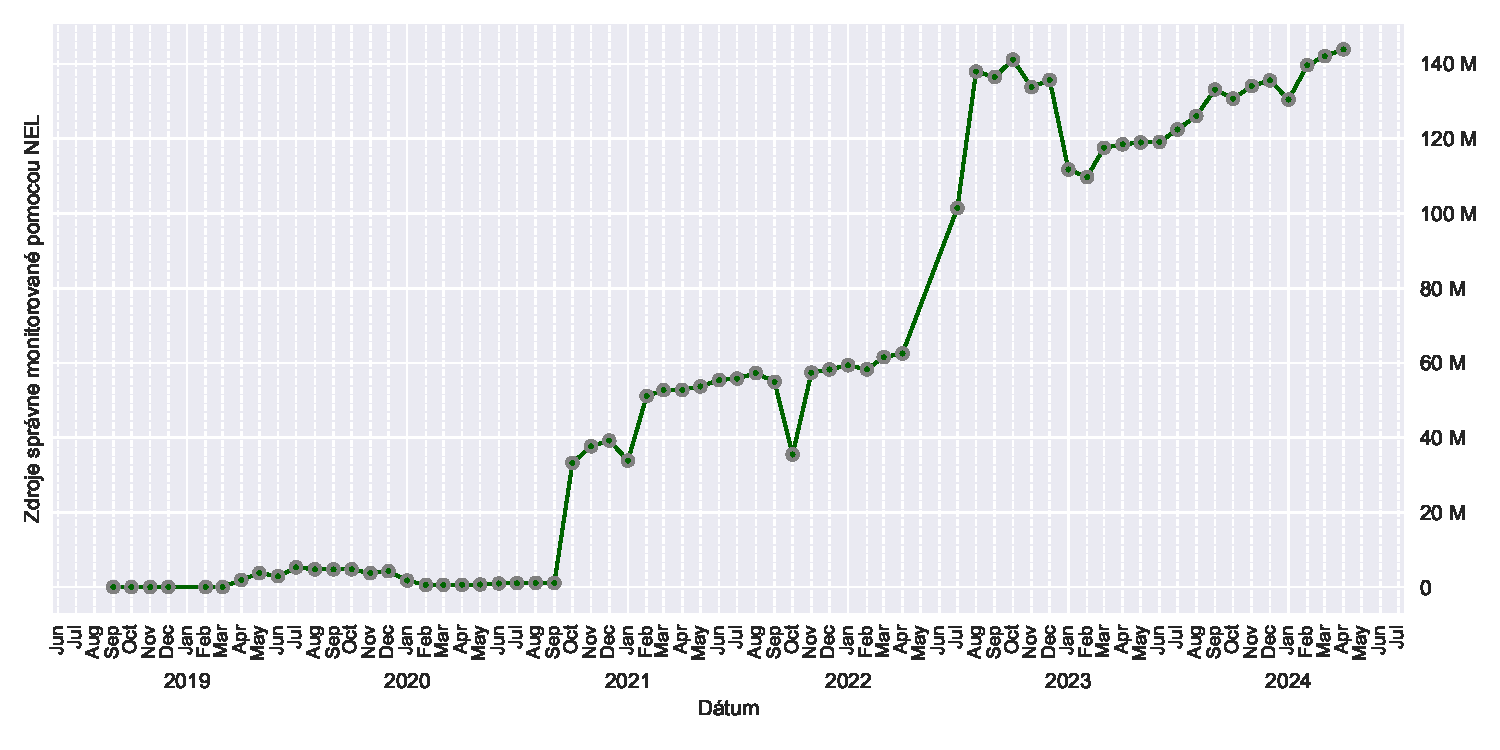
\includegraphics[scale=0.59]{obrazky-figures/httparchive_nel_deployment_resources.pdf}
 \caption{Graf zobrazujúci rast počtu monitorovaných zdrojov na doménach so správne nasadenou technológiou NEL.}
 \label{fig:httparchive-nel-deployment-resources}
\end{center}
\end{figure}

Pri zdrojoch dostupných na jednotlivých doménach som sa zameral na zistenie pomeru počtu monitorovaných zdrojov k celkovému počtu zdrojov dostupných na danej doméne.
Moje zistenia znázorňuje obrázok \ref{fig:httparchive-nel-monitored-resources-precentage-dist} --- prevažná väčšina domén monitoruje všetky zdroje.

\begin{figure}[!htb]
\begin{center}
 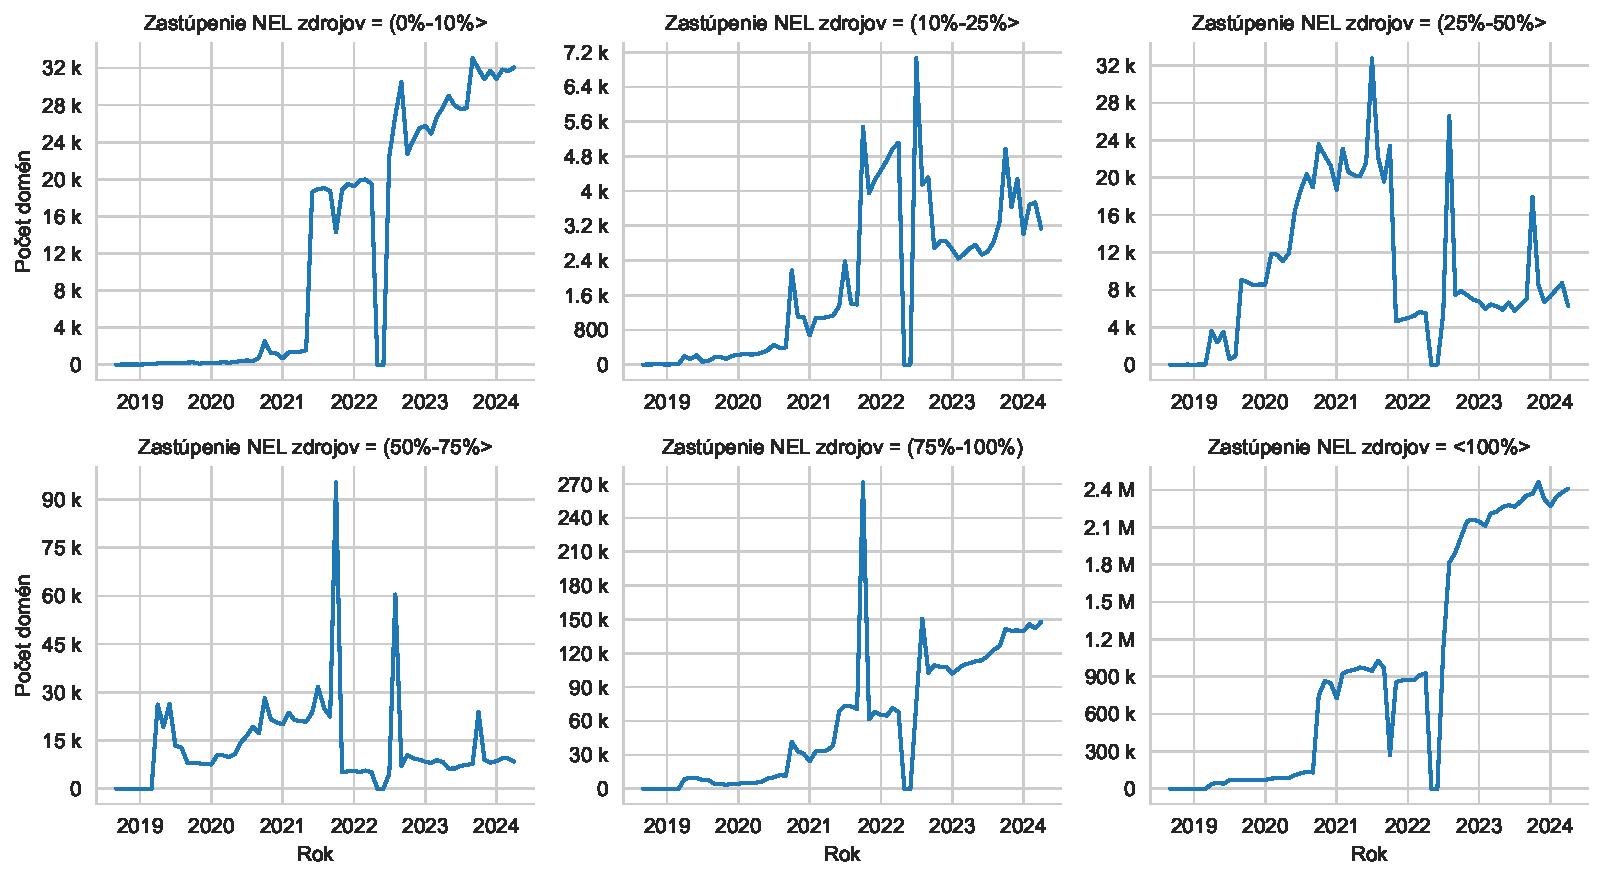
\includegraphics[scale=0.56]{obrazky-figures/httparchive_nel_monitored_resources_percentage_dist.pdf}
 \caption{Počty domén s nasadeným NEL podľa percenta monitorovaných zdrojov.}
 \label{fig:httparchive-nel-monitored-resources-precentage-dist}
\end{center}
\end{figure}

\subsection{Detekcia rôznych konfigurácií na skúmaných doménach}

Vďaka tomu, že sú v dátach záznamy pre viacero monitorovaných zdrojov dostupných na danej doméne, je možné tiež preskúmať, či doména využíva jednu, alebo viac variácií konfigurácie NEL.
Zistenia uvádza obrázok \ref{fig:httparchive-nel-config-variations}.
Najviac zastúpené sú prípady, kde dané domény používajú iba jednu konfiguráciu pre všetky svoje zdroje.
Avšak, naprieč skúmaným obdobím som identifikoval značný počet domén, ktoré používali aspoň dve rôzne konfigurácie.
Domén, ktoré využívali viac ako dve bolo veľmi málo.
Zistil som však, že maximálny počet rozdielnych NEL konfigurácií na jednotlivých doménach bol až 7.

\begin{figure}[!htb]
\begin{center}
 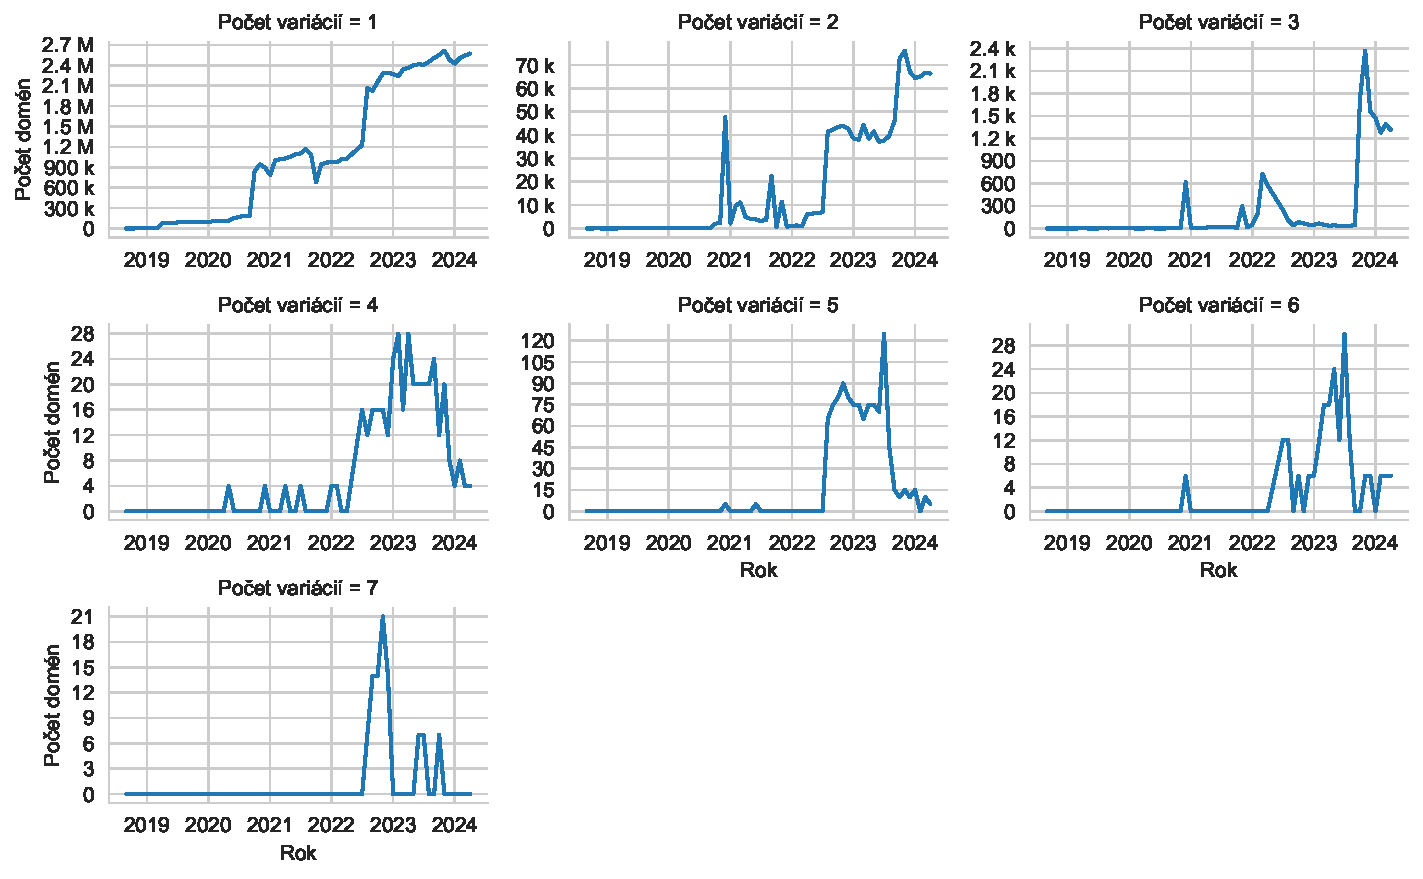
\includegraphics[scale=0.63]{obrazky-figures/httparchive_nel_config_variability_dist.pdf}
 \caption{Počty domén s nasadeným NEL podľa výskytu rozdielnych variácií použitých NEL konfigurácií na nich.}
 \label{fig:httparchive-nel-config-variations}
\end{center}
\end{figure}


% \begin{table}[!htb]
% \centering
% \resizebox{\textwidth}{!}{\begin{tabular}{l||r|r|r|r|r|r|r}
% \toprule
% Dátum & Dec 2018 & Dec 2019 & Dec 2020 & Dec 2021 & Dec 2022 & Dec 2023 & Apr 2024 \\
% Počet variácií &  &  &  &  &  &  &  \\
% \midrule
% \midrule
% 1 & 375 & 91,355 & 899,292 & 970,362 & 2,293,385 & 2,484,009 & 2,574,899 \\
% 2 & 2 & 16 & 47,796 & 784 & 42,664 & 67,124 & 66,372 \\
% 3 & 0 & 6 & 615 & 15 & 51 & 1,563 & 1,317 \\
% 4 & 0 & 0 & 4 & 0 & 12 & 8 & 4 \\
% 5 & 0 & 0 & 5 & 0 & 80 & 10 & 5 \\
% 6 & 0 & 0 & 6 & 0 & 6 & 6 & 6 \\
% 7 & 0 & 0 & 0 & 0 & 14 & 0 & 0 \\
% \bottomrule
% \end{tabular}}
% \caption{Počty domén s rôznym počtom rozdielnych NEL konfigurácií pre vybrané dátumy.}
% \label{tab:nel-config-variations}
% \end{table}

\subsection{Použitie NEL podľa typu monitorovaných zdrojov}

V rámci skúmania zdrojov som tiež preveril, aké bývajú ich typy.
Obrázok \ref{fig:httparchive-nel-resource-types-dist} predstavuje graf rozdelenia počtov zdrojov podľa ich typu.
Zistil som, že sa NEL využíva najviac na monitorovanie obrázkov, skriptov a kaskádových štýlov CSS.
Toto zistenie však možno doplniť predošlým zistením, že domény zväčša monitorujú všetky svoje zdroje.
Vzhľadom na to som usúdil, že toto skôr poukazuje na skutočnosť, že sa tieto typy zdrojov skrátka vyskytujú najčastejšie.

Sekcia \ref{crawling-results} však obsahuje o niečo špecifickejšie zistenia v kontexte s používaním NEL podľa typov monitorovaných zdrojov. 

\begin{figure}[!htb]
\begin{center}
 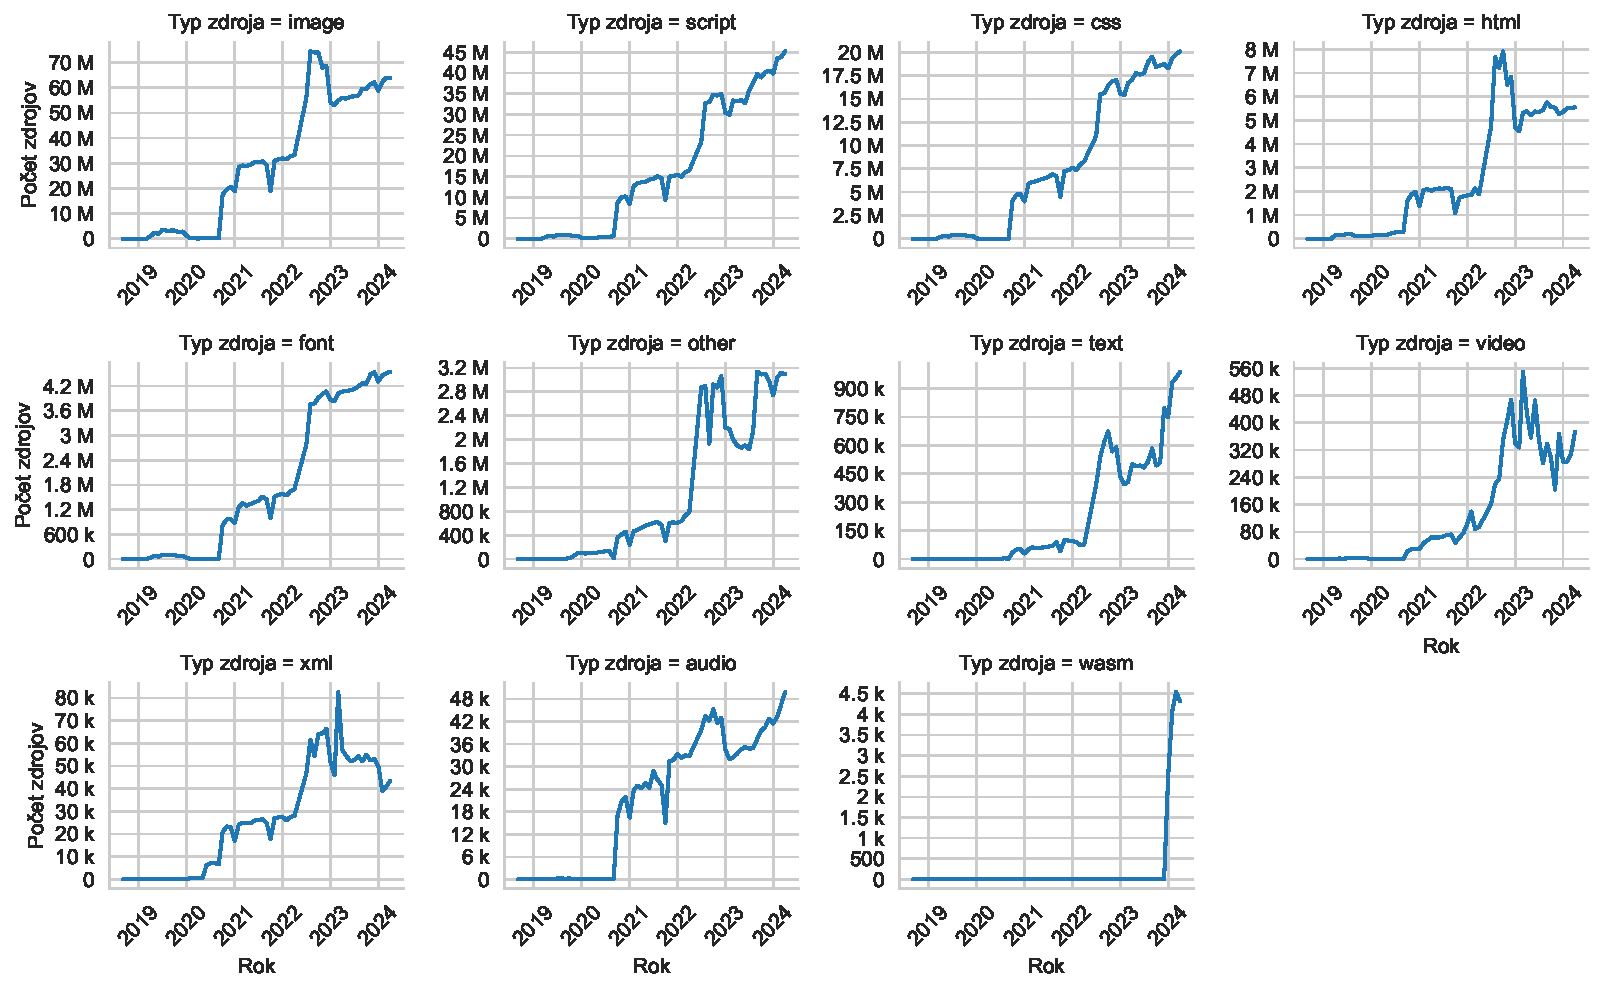
\includegraphics[scale=0.56]{obrazky-figures/httparchive_nel_resource_types_dist.pdf}
 \caption{Počty NEL monitorovaných zdrojov podľa ich typu.}
 \label{fig:httparchive-nel-resource-types-dist}
\end{center}
\end{figure}

\pagebreak



\subsection{Domény s nesprávne nasadeným NEL}

Posledným údajom vypočítaným čisto z dát HTTP Archive je vývin počtu domén s nesprávne nasadeným NEL počas skúmaného obdobia.
Zistil som, že počet týchto domén je zanedbateľný v porovnaní s počtom domén so správne nasadeným NEL.
Napríklad, \mbox{v poslednom} skúmanom mesiaci bol počet domén s nesprávne nasadeným NEL 2 564. 
Toto číslo predstavuje 0,098\% domén z celkového počtu domén, na ktorých som vtedy NEL detegoval (2 611 106), pričom počet domén so správne nasadeným NEL bolo 2 608 542.

Dodnes sa teda stále vyskytujú domény, ktoré v HTTP odpovediach zasielajú hlavičku NEL, ale nejakým spôsobom to vykonávajú nekorektne.
Pri prehliadaní HTTP Archive dát \mbox{v BigQuery} som zistil, že častým prípadom bolo vynechanie HTTP hlavičky \code{Report-To} alebo zle pomenované polia v hlavičke \code{NEL} (napríklad zamenené znaky \code{'\_'} za \code{'-'}). 
\mbox{Obrázok \ref{fig:httparchive-nel-deployment-incorrect}} znázorňuje vývoj v počte domén s nesprávne nasadeným NEL.

\begin{figure}[!htb]
\begin{center}
 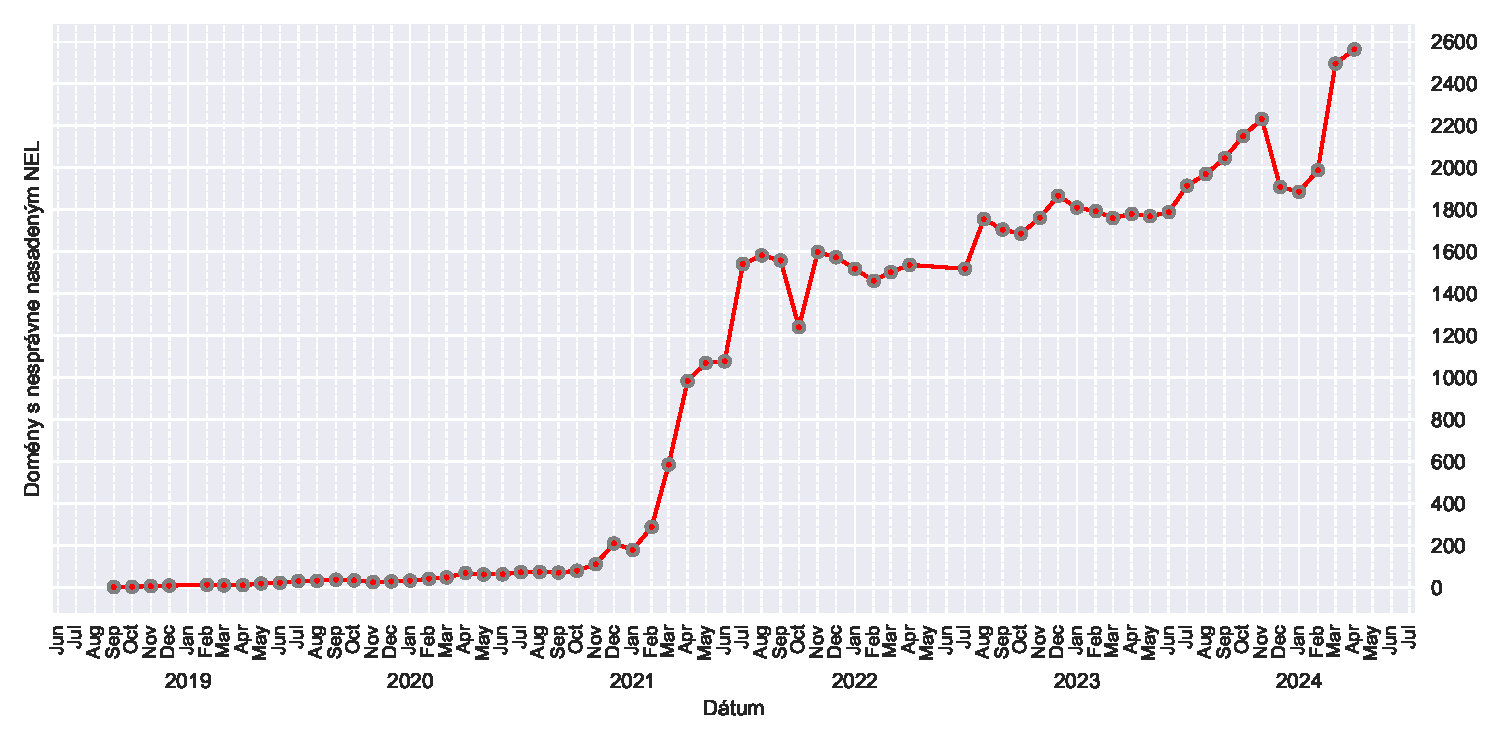
\includegraphics[scale=0.59]{obrazky-figures/httparchive_nel_deployment_incorrect.pdf}
 \caption{Graf zobrazujúci rast počtu domén s nesprávne nasadenou technológiou NEL.}
 \label{fig:httparchive-nel-deployment-incorrect}
\end{center}
\end{figure}

\pagebreak


\section{Výsledky z automatizovaného prehliadania webu}
\label{crawling-results}

Po dokončení analýzy pomocou HTTP Archive dát som množinu skúmaných domén pre hĺbkový prieskum zostavil aplikovaním dvoch kritérií na domény zahrnuté v poslednom analyzovanom mesiaci. 
Kritéria pre výber cieľových domén boli:
\begin{enumerate}
    \item Musia mať dostupných aspoň 20 NEL monitorovaných zdrojov.
    \item Musia sa objavovať v rebríčku populárnych domén TRANCO za uvedený mesiac.
\end{enumerate}
Kritéria som vybral tak, aby som mohol skúmať dostatočne veľkú vzorku zdrojov na doméne, pričom by bola šanca, že tam NEL detegujem.
Okrem toho som sa rozhodol použiť tu TRANCO aby som redukoval počet domén na prieskum, pričom ponechám v množine skúmaných tie najviac relevantné.
Zámerom redukcie bolo pracovať iba s takým množstvom domén, ktoré stihnem spracovať skriptom spomínaným v sekcii \ref{crawl_and_store}.

Aplikovaním týchto kritérií som z dát pre apríl 2024 vybral celkovo 58 596 cieľových domén pre prieskum. 
Výsledné dáta z vlastného skriptu na prehliadanie webu sa mi podarilo získať pre 33 070 domén z nich. 
Dáta pre zvyšných 25 526 domén som získať nestihol.
Zapríčinil to fakt, že dáta pre posledný analyzovaný mesiac som získal až v neskoršom štádiu práce (viď sekciu \ref{result-data}).
Tým, že je proces automatizovaného prehliadania webu relatívne pomalý, nestihol sa dokončiť pre všetky cieľové domény.

\subsubsection{Domény s nasadeným NEL}

Z celkového počtu domén, 33 070 sa úspešne podarilo získať dáta iba z 23 183 z nich.
Prehliadanie zvyšných 9 987 domén skončilo chybou alebo presmerovaním na inú doménu. 
Zo všetkých úspešne prehliadaných domén malo správne nasadený NEL 23 083 z nich.
Takže nesprávne nasadený NEL má práve 100 domén a nasadenie NEL je v tomto prípade 99.57\%.
Oproti HTTP Archive dátam je teda pokles v nasadení NEL približne iba 0.43\%.
Ako poskytovatelia NEL kolektorov boli pre skúmané domény najviac zastúpení \code{cloudflare.com} a \code{heroku.com}.

\subsubsection{Hĺbkové skúmanie vybraných domén}

Totálny počet monitorovaných zdrojov na prehliadaných doménach bol 3 962 754.
HTTP Archive dáta obsahovali pre každú doménu priemerne 7 na nej monitorovaných zdrojov.
Vo výstupných dátach \mbox{z môjho} skriptu to bolo priemerne 172 monitorovaných zdrojov pre každú doménu.  
Tento očakávaný rozdiel možno považovať za dôkaz splnenia predsavzatého cieľa vytvoriť nástroj pre hĺbkové skúmanie vybratých domén. 
Mojim skriptom totiž prehliadam zhruba 24.5krát viac monitorovaných zdrojov v porovnaní s projektom HTTP Archive.
To ale zároveň znamená, že proces prehliadania každej domény trvá pomerne dlho.

Počet zdrojov typu \code{html} v porovnaní s HTTP Archive dátami markantne stúpol.
Pre porovnanie, najzastúpenejšie typy monitorovaných zdrojov boli:
\begin{enumerate}
    \item \code{image} -- 2 457 577 zdrojov,
    \item \code{script} -- 483 698 zdrojov,
    \item \code{html} -- 482 927 zdrojov, pričom došlo k značnému nárastu oproti zdrojom typu \code{css},
    \item \code{css} -- 312 895 zdrojov.
\end{enumerate}

Prevažná väčšina skúmaných domén (98.95\%) monitorovala svoje zdroje pomocou jedinej konfigurácie NEL. 
Až na jeden prípad s troma konfiguráciami NEL, všetky zvyšné domény používali práve dve konfigurácie NEL.
Na týchto možno skúmať stratégie využitia NEL podľa typu zdrojov hlbšie.

Zistil som, že tieto domény používajú jednu konfiguráciu pre majoritu svojich zdrojov \mbox{a druhú} pre menšiu množinu \textit{vybraných} zdrojov.
Medzi hlavné zdroje väčšinou patrila domovská webstránka spolu s jednoznačnou väčšinou ostatných dostupných webstránok, obrázkov a štýlov CSS.
Napríklad, na doméne \code{comparepower.com} som našiel väčšinovú konfiguráciu pre všetky monitorované webstránky a obrázky so 100\% hlásením zlyhaní \mbox{a 1\% hlásením} úspechov. 
Táto konfigurácia tiež obsahovala prevažnú majoritu monitorovaných skriptov.
Druhá konfigurácia obsahovala ďalších 22 skriptov a tiež 7 zdrojov typu \code{font},
pričom bola nastavená na hlásenie všetkých zlyhaní a žiadnych úspechov.
Takéto rozdelenie konfigurácie bolo v dátach najčastejšie.

Iným častým rozdelením bolo rozdelenie na konfiguráciu pre zdroje samotnej domény a konfiguráciu pre statický skript prevzatý od poskytovateľa kolektorov \code{cloudflare.com}, ktorý bol uložený na skúmanej doméne.
Pravdepodobne teda ide o sekundárnu konfiguráciu vytvorenú používaním konkrétnej služby od poskytovateľa \code{cloudflare.com}.

Tiež sa vyskytovali prípady, v ktorých pre zdroje typu \code{html} bola jedna konfigurácia nastavená na monitorovanie 5\% chýb a 0.5\% úspechov prevažnej väčšiny zdrojov.
Tieto zdroje boli ale paradoxne práve tie hlavné zdroje danej domény ako napríklad aj domovské stránky.
Takáto konfigurácia bola charakteristická pre poskytovateľa \code{heroku.com}.
Doplňujúcou konfiguráciou pre tieto prípady bola napríklad pre doménu \code{nuovopay.com} konfigurácia monitorujúca webstránky obsahujúce hlavne informatívny obsah.
Tento obsah však bol monitorovaný pre 100\% zlyhaní a 0\% úspechov.

Je náročné jednoznačne určiť konkrétnu stratégiu, s ktorou si domény vyberajú rôzne konfigurácie pre rôzne typy svojich zdrojov.
Zistil som však, že samotné nastavenie konfigurácií, ktoré som preskúmal, prevažne závisí od použitého poskytovateľa NEL kolektorov.
V prípadoch, že obe konfigurácie využívali \code{cloudflare.com} kolektor, jedna bola nastavená pre hlavné zdroje domény a druhá pre tie vedľajšie, najčastejšie skripty prevzaté od samotného cloudflare.
Domény využívajúce aj \code{heroku.com}, aj \code{cloudflare.com}, rozdelili svoje zdroje tak, aby na \code{heroku.com} boli zasielané hlásenia menej často, pričom sledovali aj úspechy, no na \code{cloudflare.com} zasielajú všetky zlyhania vybraných zdrojov bez ohľadu na úspechy. 
Konfigurácie používajúce iných poskytovateľov NEL kolektorov boli vždy spárované s buď \code{cloudflare.com}, alebo s \code{heroku.com}, pričom počet ich výskytov bol v dátach zanedbateľný.
